\documentclass{beamer}


\usetheme{Warsaw}
\usecolortheme{crane}


\title{Solving Equations}
\subtitle{Mathematical Methods in the Physical Sciences}
\author{Steve Mazza}
\institute[Naval Postgraduate School]
{ 
    Naval Postgraduate School \\
    Monterey, CA \\
    
\includegraphics[height=3cm]{images/NPS_logo.jpg}
}
\date {SE3030, Winter/2014 \\ Quantitative Methods of Systems Engineering}
\subject{Quantitative Methods of Systems Engineering}


\begin{document}

\frame{\titlepage}


\frame{{Introduction}
	\begin{center}
		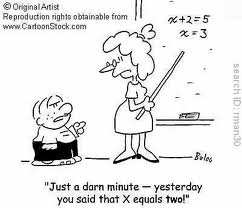
\includegraphics[scale=0.75]{images/algebraCartoon.jpg}
	\end{center}
}


\frame{{Solving an Equation in One Variable}
	Given an equation of the form $f(x)=0$, we want to find a solution to within the accuracy of our computations.
	We explore four methods
	\begin{itemize}
		\item Newton's Method, which uses a series of linear approximations by taking the derivative
		\item Poor Man's Newton, which uses a series of linear approximations without taking the derivative (numerical approximation).
		\item Another linear method that uses bracketing
		\item Divide and Conquer, which looks a little like a binary search
	\end{itemize}
}


\frame{{Newton's Method}
	\begin{block}{Newton-Raphson}
		\[x_{n+1} = x_n - \frac{f(n)}{f'(n)}\]
	\end{block}
	\begin{center}
		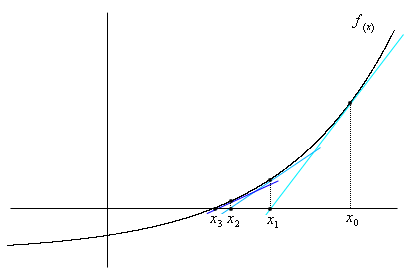
\includegraphics[scale=0.4]{images/newton_method_graph.png}
	\end{center}
	Geometrically, $(x_{n+1}, 0)$ is the intersection with the $x$-axis of the tangent to the graph of $f$ at $(x_n, f (x_n))$.
}


\frame{{Newton's Method Example}
	We calculate $\sqrt{5}$ by finding an approximate solution to the equation $f(x) = x^2-5 = 0$.  We choose a first approximation of $x_0=2$, so
	\begin{align*}
		f(x) &= x^2-5 \\
		f'(x) &= 2x \\
		fLx_0(x) &= f(x_0) + f'(x_0)(x-x_0) \\
		&= -1+4(x-2) \\
		&= 4x-9 = \frac{9}{4} = 2.25 \\
		fLx_1(x) &= f(x_1) + f'(x_1)(x-x_1) \\
		&= \left(\frac{81}{16}-5\right)+\frac{9}{2}\left(x-\frac{9}{4}\right) \\
		&= \frac{9}{2}x-\frac{161}{16} = 2.236111
	\end{align*}
}


\frame{{Newton's Method Caveats}
	\begin{itemize}
		\item Many functions have more than one zero
		\item Some functions will never converge
		\item Unfortunate initial guesses can be very misleading
		\item If $f$ is implicitly defined, we may find values for $x_n$ for which $f$ is undefined.
	\end{itemize}
	However, if $f$ goes from negative to positive at the true solution $x$, and $f'$ is increasing between $x$ and your guess $x_0$, which is greater than $x$, then the method will always converge.
}


\frame{{Poor Man's Newton}
	Instead of calculating the derivative at each successive step we use the following approximation
	\begin{block}{Approximation to the Derivative}
		\[f'(x) \approx \frac{f(x_i+d)-f(x_i)}{d}\]
	\end{block}
	Then in general,
	\begin{block}{Approximation to Newton}
		\[x_{n+1} = x_n-d\frac{f(x_n)}{f(x_n+d)-f(x_n)}\]
	\end{block}
	The trick is selecting an appropriate value for $d$.
}


\frame{{Another Linear Method}
	This method almost always converges but can be painfully slow.
	\begin{itemize}
		\item Select two values which you assume to be near the solution of interest.
		\item Evaluate the function at the two arguments.
		\item Draw a straight line through the solutions, noting where the line hits the $x$-axis.
		\item Use the $x$-intercept to replace one of the two original values.
	\end{itemize}
	One of two outcomes are possible.
	\begin{itemize}
		\item Values of the two arguments have the same sign.  In this case, replace the old argument furthest from the new one.
		\item Values of the two arguments have different signs.  In this case, replace the old argument with the same sign as the new one.
	\end{itemize}
	We approximate the derivative in Newton's method by using values at the previous two guesses, rather than by the last guess and it plus $d$, as in Poor Man's Newton.
}


\frame{{Divide and Conquer}
	This method provides some improvement in speed for worst cases over the previous method by replacing one of the old arguments with the \emph{middle} as opposed to the $x$-intercept.  This is only productive after your solutions have achieved opposite signs.
	\begin{itemize}
		\item Select two arguments, $a$ and $b$.
		\item Evaluate $f(a)$, $f(b)$, and $f\left(\dfrac{a+b}{2}\right)$.
		\item Replace either $a$ or $b$ with the middle value.  Replace the original value with the same sign as the middle value.
	\end{itemize}
	This is slow compared to Newton's best case performance, however it guarantees steady progress toward a solution and so generally is an improvement over the previous two methods.
}


\frame{{Solving Two General Equations in Two Variables}
	We can generalize Newton's Method in two (or more) dimensions as follows.
	\begin{itemize}
		\item Assume two functions, $f$ and $g$, in two variables, $x$ and $y$, such that $f(x,y)=0$ and $g(x,y)=0$.
		\item Compute the gradients of $f$ and $g$ at some initial point.
		\item Find a new point at which the linear approximations to $f$ and $g$ defined by the gradients at the initial point are both 0.
		\item Iterate.
	\end{itemize}
	This works just as well as Newton does in one dimension with the additional caveat that there may be no solution to the equations (i.e., the curves for $f$ and $g$ may not intersect).
}

\frame{{Questions?}
	\begin{center}
		
\includegraphics[width=.7\textwidth]{images/fin.png}
	\end{center}
}

\end{document}
